\documentclass{article}

\usepackage{graphicx}
\usepackage{indentfirst}
\usepackage{booktabs}
\usepackage[a4paper, total={6in, 8in}]{geometry}
\usepackage{hyperref}
\usepackage{fancyhdr}
\usepackage{xepersian}
\usepackage{fontspec}
\usepackage{url}
\settextfont[Scale=1.2,ExternalLocation=fonts/,BoldFont=B Nazanin Bold.ttf]{B Nazanin}
\setlatintextfont[Scale=1.2,ExternalLocation=fonts/,BoldFont=XB Zar.ttf]{Times New Roman}

\begin{document}


%title page%
\begin{titlepage}
	\begin{center}
		\vspace{0.2cm}
		
		
\includegraphics[width=0.4\textwidth]{sharif.png}\\
		\vspace{0.5cm}
		\textbf{ \Huge{فاز دوم}}\\
		\vspace{0.25cm}
		\textbf{ \Large{پروژه مقدمه‌ای بر بیوانفورماتیک \\ دکتر علی  شریفی‌زارچی و دکتر سمیه کوهی}}
		\vspace{0.2cm}
		
		
		\large \textbf{دانشکده مهندسی کامپیوتر}\\\vspace{0.1cm}
		\large   دانشگاه صنعتی شریف\\\vspace{0.2cm}
		\large   ﻧﯿﻢ‌سال اول ۰۱-۰۲ \\\vspace{0.2cm}
		\large{\Large{امیرحسین باقری - 98105621}}\\
		\large{\Large{مهدی مستانی - 97100513}}\\
		\large{\Large{محمدرضا مفیضی - 98106059}}\\
	\end{center}
\end{titlepage}
%title page%

\newpage
\tableofcontents
\newpage
%pages header
\pagestyle{fancy}
\fancyhf{}
\fancyfoot{}
\setlength{\headheight}{59pt}
\cfoot{\thepage}
\lhead{فاز دوم}
\rhead{
\includegraphics[width=0.1\textwidth]{sharif.png}\\
		دانشکده مهندسی کامپیوتر
}
\chead{پروژه مقدمه‌ای بر بیوانفورماتیک}
%pages header

\section{بیان ژن‌ها}
در جدول \ref{tab:genes} ژن‌هایی که بیان آن‌ها به طرز معناداری بین گروه سالم و گروه بیماران متفاوت است را نمایش می‌دهیم
\footnote{جدول کامل به همراه این گزارش ضمیمه شده است.}.

\begin{table}[h!]
	\begin{latin}
		\begin{center}
			\begin{tabular}{@{}cccc@{}}
				\toprule
				Gene Symbol & Gene ID & Adj. P-Val & logFC  \\ \midrule
				MPO         & 4353    & 3.617e-19 & -5.563 \\
				FLT3        & 2322    & 4.835e-19 & -5.250 \\
				KIAA0101    & 9768    & 6.308e-19 & -4.559 \\
				BUB1B       & 701     & 1.664e-18 & -2.756 \\
				SUCNR1      & 56670   & 1.938e-18 & -2.996 \\ \bottomrule
			\end{tabular}
		\end{center}
	\end{latin}
	\label{tab:genes}
	\caption{5 ژنی که بیان آن‌ها به طرز معناداری بین گروه سالم و گروه بیماران متفاوت است.}
\end{table}

حالا ژن‌هایی که در بیماران از بقیه بیشتر بیان شده‌اند و همچنین ژن‌هایی که کمتر از بقیه بیان شده‌اند را در جدول \ref{tab:up-down} نمایش می‌دهیم
\footnote{جدول کامل این بخش هم به همراه این گزارش ضمیمه شده است.}.

\begin{table}[h!]
	\begin{latin}
		\begin{center}
			\begin{tabular}{@{}cc@{}}
				\toprule
				Most Expressed & Least Expressed \\ \midrule
				STK38          & MPO             \\
				CBX7           & FLT3            \\
				PLCL2          & KIAA0101        \\
				PECR           & BUB1B           \\
				HLA-F          & SUCNR1          \\ \bottomrule
			\end{tabular}
		\end{center}
	\end{latin}
	\label{tab:up-down}
	\caption{5 ژنی که در بیماران بیشتر/کمتر از بقیه بیان شده‌اند.}
\end{table}

\section{بررسی \lr{pathway} و \lr{gene ontology}}
با رفتن به سایت \href{https://maayanlab.cloud/Enrichr/}{\lr{enrichr}} و قرار دادن لیست ژن‌های بیشتر بیان‌شده (شکل \ref{fig:enrichr}) آن‌‌ها را بررسی می‌کنیم.
\begin{figure}[h!]
	\centering
	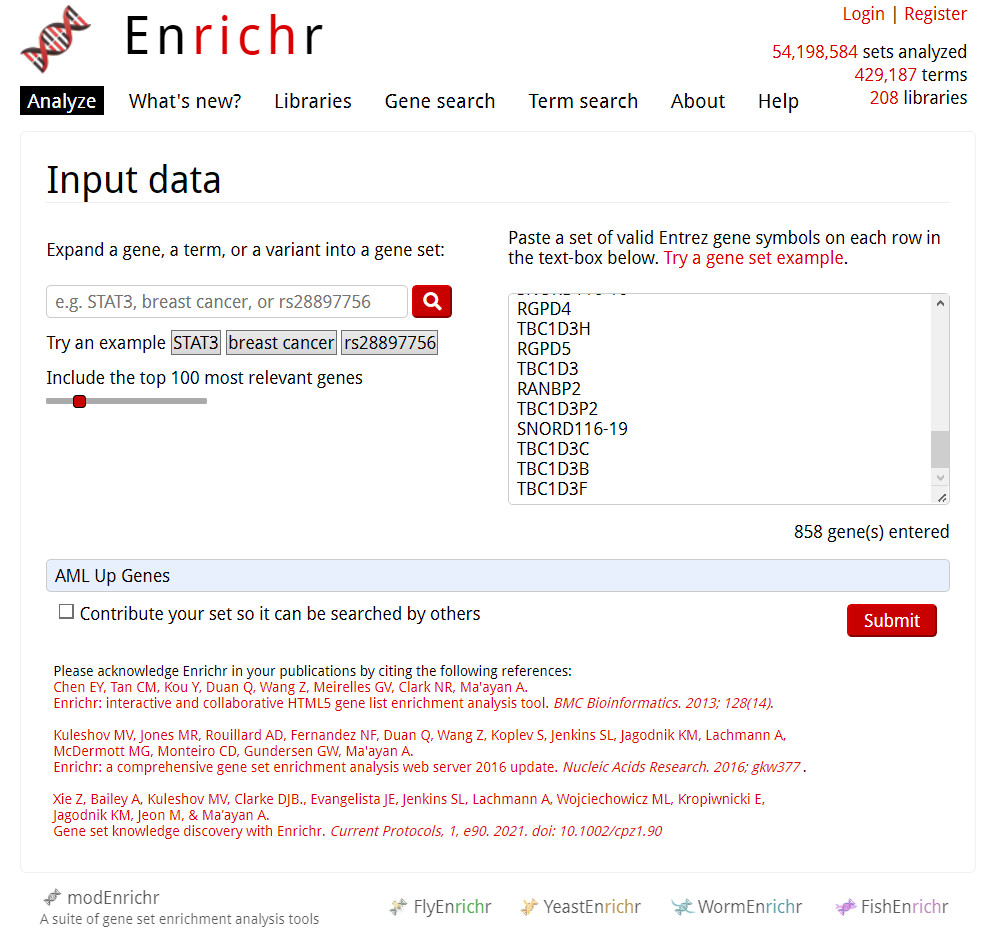
\includegraphics[width=0.5\columnwidth]{figs/enrichr.jpg}
	\caption{وارد کردن داده‌ها برای شروع آنالیز}
	\label{fig:enrichr}
\end{figure}



\clearpage

\begin{thebibliography}{99}
	\begin{latin}
		\bibitem{nature-microarray}
		Nature Defenition Microarray (2014), Nature Education, \url{https://www.nature.com/scitable/definition/microarray-202}
		
%		\bibitem{lamport94
%		Leslie Lamport (1994) \emph{\LaTeX: a document preparation system}, Addison
%		Wesley, Massachusetts, 2nd ed.
	\end{latin}
\end{thebibliography}



\end{document}
